\section{Programming languages}
\subsection{Definition of programming language}
A programming language is defined by:
\begin{itemize}
    \item \emph{syntax}: is the form of programs, how to write them, expressions, commands and various constructs.
    It's formally defined in the language specification via a formal grammar.
    A lexical grammar for tokens which is a regular grammar and a syntactic grammar for the language constructs, which is a context free grammar.
    Those specifications are used by the compiler for scanning and parsing of the source code.

    \item \emph{semantics}: it's the meaning of the syntax, what the constructs means and do.
    It's described precisely in an informal way so it can leave ambiguities.    

    \item \emph{pragmatics}: is the way in which the pl is intended to be used in practice. It includes coding conventions and guidelines for elegant structuring of code, basically it's the language best practice.
    It also includes the description of the supported programming paradigms (it's OOP, it's functional, ecc, ecc).
\end{itemize}

\subsection{Programming paradigms}
A paradigm is a style of programming, it's a set of key concepts and abstraction provided by the language.
Eg:
\begin{itemize}
    \item \emph{imperative programming} brings us variables and procedures;
    \item \emph{OOP}: means objects, methods and classes;
    \item \emph{functional programming}: means values, expressions, functions, high-order functions;
    \item \emph{logic programming}: assertions, relations;
    \item \emph{concurrent programming}: processes, communication, synchronization.
\end{itemize}

\subsection{Implementation of a PL}
A program written in language $L$ must be executable, to achieve that every language defines an \emph{abstract machine} $M_L$ having $L$ as machine language.
In order to execute $L$ over an host machine $M_O$ (which doesn't necessarily understand $L$) we use techniques like \emph{compilation} or \emph{interpretation} (or both).

The abstract machine $M_L$ is a collection of data structures and algorithms which can perform the storage and execution of programs written in $L$, so it is an abstraction for the underlying hardware machine.
The basic structure for such abstract machine has:
\begin{itemize}
    \item memory: in which resides programs instructions and data;
    \item interpreter: stuff for the data processing, sequence control, memory management, ecc
\end{itemize}

\begin{figure}[H]
    \centering
    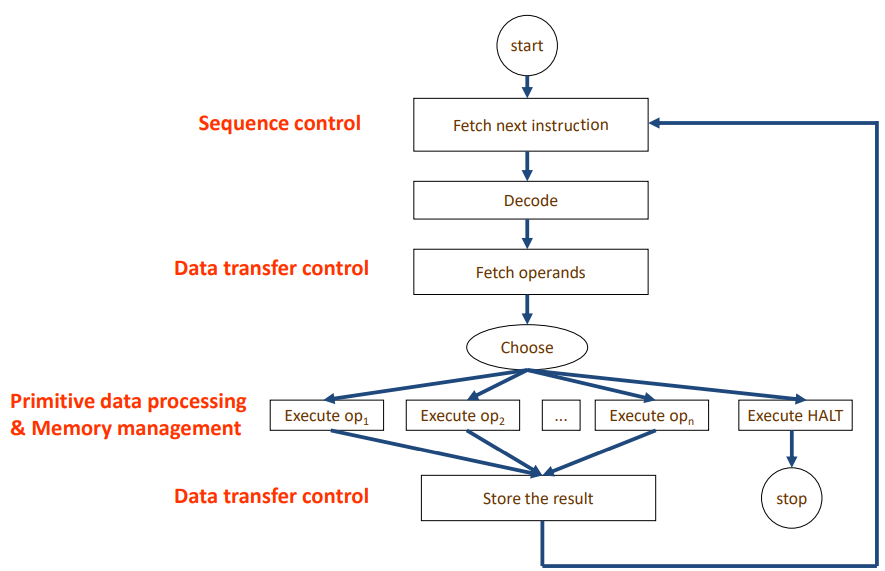
\includegraphics[width=380px]{images/1_Introduction/interpreter.png}
    \caption{General structure of an interpreter}
\end{figure}

Each abstract machine $M$ defines a proper language $L_M$ which includes all the programs which can be executed by the interpreter of $M$.
Moreover programs are data on which the interpreter can act in order to execute the actual program and the various components of $M$ corresponds to the components of $L_M$, for example:
\begin{itemize}
    \item primitive data processing of $M$ corresponds to primitive data types of $L_M$;
    \item sequence control of $M$ corresponds to control structures of $L_M$;
    \item data transfer control of $M$ corresponds to parameter passing and return value of $L_M$;
    \item memory management of $M$ corresponds to memory management of $L_M$.
\end{itemize}

\subsubsection{JVM}
It's an example of abstract machine whose language is the Java bytecode.
It's memory is mainly composed by heap, stack and permanent storage and it' execution model is an interpreter.
The core of the JVM is basically:
\begin{verbatim}
do {
    byte opcode = <fetch an opcode>
    switch (opcode) {
    case opCode1:
        <fetch operands for opCode1>
        <execute action for opCode1>
        break
    case opCode2:
        <fetch operands for opCode2>
        <execute action for opCode2>
        break
    case ...
} while (<more to do>)
\end{verbatim}


\subsection{Implementing an abstract machine}
Abstract machine can be implemented in hardware or in firmware but in hardware it's not so convenient in general for the high-level concepts it needs to handle.

An abstract machine $M$ can be implemented over an host machine $M_O$ using the component of $M_O$ and it's machine language to realize the ones in $M$.
We have two main cases:
\begin{itemize}
    \item $M$ is an extension of $M_O$ in which the interpreter of $M$ coincides with the interpreter of $M_O$ but has more constructs so some components can differ;
    \item $M$ is interpreted over $M_O$ in which the interpreter of $M$ coincides with the interpreter of $M_O$ but some components of the machines can coincide.
\end{itemize}

Of course machines can be nested building an actual hierarchy.

\subsection{Compilation and interpretation}
\subsubsection{Pure interpretation}
We have an host machine $M_O$ which understands and executes the $L_O$ language.
In $L_O$ we build an abstract machine $M_L$ for the language $L$.

So we have that $M_L$ is interpreted over $M_O$, this approach of course is not very efficient mainly because of the interpreter loop but the interpretation leads to better diagnostics and debugging because the interpreter has more context of the execution.

\subsubsection{Pure compilation}
We \emph{translate} programs written in $L$ into equivalent programs written in $L_O$ which is the machine language of $M_O$.
As a result the translated program can be executed directly on $M_O$.

The execution is of course more efficient but it needs that translation process (compilation) and the produced code is usually larger than the original one.
Moreover during the compilation phases the compiler can fix decisions in order to avoid to make them at run time, for example it can execute type checking in order to avoid type mismatch during the execution or it can allocate variables statically without the need for the lookup at run time.
In the end the compiler can optimize the produced code in order to exploit hardware features.

\subsubsection{Hybrid approach}
All modern implementation of programming languages use both techniques.
We have at least:
\begin{itemize}
    \item compilation from a language to machine code;
    \item interpretation for the I/O operations (basically we ask run time support to the OS for such operations).
\end{itemize}

This approach can be modeled by an \emph{intermediate abstract machine} $M_I$ whose language is $L_I$.
Then we compile from the language $L$ to the language $L_I$ which is then interpreted by $M_I$.

\subsubsection{Static and dynamic linking}
In static linking the library routines are merged with the object code of the program, so they are embedded in the resulting binary executable.

In dynamic linking though external libraries (windows .dll, linux .so) are linked at run-time by the loader (using stubs in the executable).

\subsection{Virtual machines}
Several language implementations adopt a compilation + interpretation schema whose intermediate machine is a \emph{virtual machine}.
Some famous implementations are:
\begin{itemize}
    \item Pascal: whose compiler produces \emph{P-Code} that can be interpreted or compiled into object code;
    \item Java: whose compiler produces \emph{bytecode} which is interpreted by the Java Virtual Machine (JVM) that can translate bytecode into machine code exploiting just-in-time compilation;
    \item C\#, F\#, ..: whose compilers generate \emph{CIL} code (Common Language Infrastructure) that can be executed in .NET, .NET core or other implementations (like Mono for Linux) that compile that intermediate representation into target machine code.
\end{itemize}

\begin{figure}[H]
    \centering
    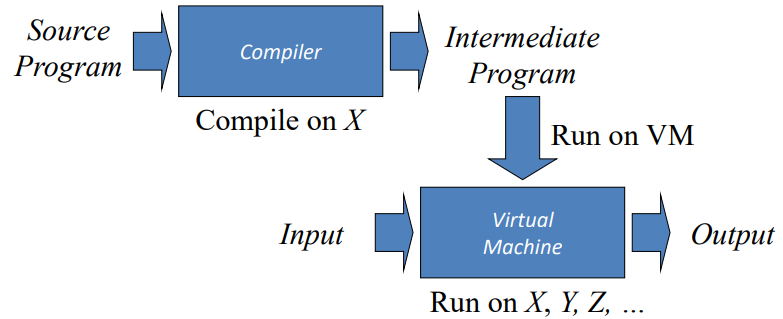
\includegraphics[width=330px]{images/1_Introduction/VM.png}
    \caption{Typical VM workflow}
\end{figure}

Some advantages of using an intermediate abstract machine are:
\begin{itemize}
    \item \emph{portability}: you compile the original code and distribute the IR that can then be executed on any platform that provides an interpreter;
    
    \item \emph{interoperability}: given a new language you just need to provide a compiler from that language to one of the IR of choose, then you can exploit the libraries that already exists for that IR.
    It's by design for Microsoft CLI and common practice for JVM (we have Scala and Kotlin which both translates to JVM bytecode);
\end{itemize}

\subsection{LLVM}
LLVM is a compiler infrastructure (a framework for compilers) with reusable libraries and well-defined interfaces.
The main concept is to use a frontend translator from the language you want to \emph{LLVM IR} (the intermedite representation of LLVM) and then use the backend you need in order to compile the LLVM IR to the target machine you like.
Moreover LLVM IR can be interpreted and is much lower-level than Java bytecodes or CIL.

\begin{figure}[H]
    \centering
    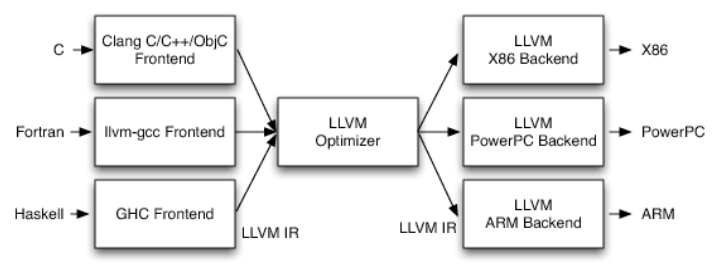
\includegraphics[width=300px]{images/1_Introduction/LLVM.png}
    \caption{LLVM workflow}
\end{figure}

\section{Runtime}
Every programming language defines an execution model which is partly implemented by the \emph{runtime system}.
The runtime system provides some useful functionality during the execution of the programs and is present both in interpreted and compiled languages in different weight.

Some parts of the runtime are:
\begin{itemize}
    \item code added by the compiler: for example in C programs the code executed before the main function is part of the runtime;
    \item code running in other threads/processes during the main program execution: for example in the memory managed languages the garbage collector executed in a different thread is part of the runtime;
    \item language libraries;
    \item OS functionalities;
    \item the interpreter/virtual machine itself.
\end{itemize}

Some runtime jobs are instead:
\begin{itemize}
    \item memory management: the push/pop of the activation record of the functions, heap allocations and garbage collection;
    \item input/output: interface with the file system provided by the OS;
    \item interaction with the runtime environment: environment variables, system registry, disk drivers, keyboards, ...;
    \item parallel execution via threads/tasks/processes;
    \item dynamic type checking and dynamic bindings;
    \item dynamic loading of dynamic libraries and modules;
    \item debugging functionalities;
    \item code generation and optimization (in JIT interpreter);
    \item verification and monitoring of resources.
\end{itemize}

